\documentclass{article}
\usepackage{bm}
\usepackage{amsmath}
\usepackage{graphicx}
\usepackage{mdwlist}
\usepackage[colorlinks=true]{hyperref}
\usepackage{geometry}
\usepackage{kotex}
\geometry{margin=1in}
\geometry{headheight=2in}
\geometry{top=2in}
\usepackage{palatino}
%\renewcommand{\rmdefault}{palatino}
\usepackage{fancyhdr}
%\pagestyle{fancy}
\rhead{}
\lhead{}
\chead{%
  {\vbox{%
      \vspace{2mm}
      \large
      Hardware System Design 4190.309A\hfill
\\
      Seoul National University
      \\[4mm]
      \textbf{Practice \#3. How to use Vivado \& Basic syntax}\\
      \textbf{Jiwon Lee, Sangjun Son}
    }
  }
}

%%%%%%%%%%%%%%%%%%%%%%%
\usepackage{xcolor}
\usepackage{listings}
\definecolor{vgreen}{RGB}{104,180,104}
\definecolor{vblue}{RGB}{49,49,255}
\definecolor{vorange}{RGB}{255,143,102}

\lstdefinestyle{verilog-style}
{
    language=Verilog,
    basicstyle=\small\ttfamily,
    keywordstyle=\color{vblue},
    identifierstyle=\color{black},
    commentstyle=\color{vgreen},
    numbers=left,
    numberstyle=\tiny\color{black},
    numbersep=10pt,
    tabsize=8,
    moredelim=*[s][\colorIndex]{[}{]},
    literate=*{:}{:}1
}

\makeatletter
\newcommand*\@lbracket{[}
\newcommand*\@rbracket{]}
\newcommand*\@colon{:}
\newcommand*\colorIndex{%
    \edef\@temp{\the\lst@token}%
    \ifx\@temp\@lbracket \color{black}%
    \else\ifx\@temp\@rbracket \color{black}%
    \else\ifx\@temp\@colon \color{black}%
    \else \color{vorange}%
    \fi\fi\fi
}
\makeatother

\usepackage{trace}
%%%%%%%%%%%%%%%%%%%%%%%

\usepackage{paralist}

\usepackage{todonotes}
\setlength{\marginparwidth}{2.15cm}

\usepackage{tikz}
\usetikzlibrary{positioning,shapes,backgrounds}

\begin{document}
\pagestyle{fancy}

\section*{Goal}

\begin{itemize*}
\item Implement base of Float32 MUL+ACC.
\item Implement Adder, Multiplier, Fused multiplier (VERILOG).
\end{itemize*}

\section{Implementation}

\subsection{Adder}

이 누산기는 2개의 input, 1개의 output, 1개의 overflow detecting bit 로 이루어져 있다.
같은 크기의 bitwidth를 가지는 2개의 input을 더했을 때, output의 bitwidth도 동일하기 때문에, overflow가 발생할 수 있다.
Overflow detecting은 concatenation assign을 통해 구현하였다.
Overflow bit와 output의 총 길이는 bitwidth+1이고, 2개의 input을 더했을 때 나올 수 있는 최대 bit수는 bitwidth+1이기 때문에, 이를 통해 overflow를 detect 할 수 있다.

\begin{lstlisting}[style={verilog-style}]
`timescale 1ns / 1ps
module my_add #(
    parameter BITWIDTH = 32
)
(
    input [BITWIDTH-1:0] ain,
    input [BITWIDTH-1:0] bin,
    output [BITWIDTH-1:0] dout,
    output overflow
);
    // concatnate (overflow, dout) & detect overflow
    assign {overflow, dout} = ain + bin;
endmodule
\end{lstlisting}


\subsection{Multiplier}
곱셈기는 2개의 input, 1개의 output으로 이루어져 있다. 곱셈기는 overflow가 발생할 일이 없다.
입력 가능한 최대 정수형 두 값을 서로 곱했을 때의 값은 아래와 같다.
\begin{equation}
\left(2^{bitwidth}-1\right) \cdot \left(2^{bitwidth}-1\right) = 2^{2 \cdot bitwidth}-2^{bitwidth+1}+1
\label{eq1}
\end{equation}

Equation~\ref{eq1}에서도 알 수 있듯이, 최대 bit수는 $2 \cdot bitwidth$이기 때문이다.

\begin{lstlisting}[style={verilog-style}]
`timescale 1ns / 1ps
module my_mul #(
    parameter BITWIDTH = 32
)
(
    input [BITWIDTH-1:0] ain,
    input [BITWIDTH-1:0] bin,
    output [2*BITWIDTH-1:0] dout
);
    assign dout = ain * bin;
endmodule
\end{lstlisting}

\subsection{Fused Multiplier}

단일 곱셈-누산기는 2개의 input, 1개의 output, en register, clk register로 이루어져 있다.
en은 현재까지의 계산결과를 저장하고 있는 register이고, clk은 계산 및 누산이 수행되는 타이밍을 결정한다.
구현은 clk이 posedge일때, en과 2개의 input을 읽어 output을 계산하였다.
en 이 1인 경우, 기존의 output과 input 2개를 곱한 값을 output에 저장하였다.
en 이 0인 경우, output을 0으로 초기화하였다.

\begin{lstlisting}[style={verilog-style}]
`timescale 1ns / 1ps

module my_fusedmult #(
    parameter BITWIDTH = 32
)
(
    input [BITWIDTH-1:0] ain,
    input [BITWIDTH-1:0] bin,
    input en,
    input clk, 
    output reg [2*BITWIDTH-1:0] dout
);
    // read en when clk is posedge
    always @(posedge clk) begin
        if(en == 1)
            dout <= dout + ain * bin;
        else 
            dout = 0;
    end
endmodule

\end{lstlisting}

\section{Results \& Conclusion}

\subsection{Adder}
testbench에서 주어지는 ain, bin의 값은 0 ~ $2^{31}-1$ 까지의 임의의 값이다.
따라서, dout의 값은 최대 $2^{31}-2$  이고, 이는 32bit로 만들 수 있는 최댓값인 $2^{31}-1$  보다 작으므로 주어진 testbench에서는 overflow가 발생하지 않는다.
하지만, 실제로 ain, bin의 값을 증가시켜 overflow가 발생하도록 하였을 때, overflow bit가 1이 되어 detecting한다는 것을 알 수 있었다.

\begin{figure}[ht]
	\centering
	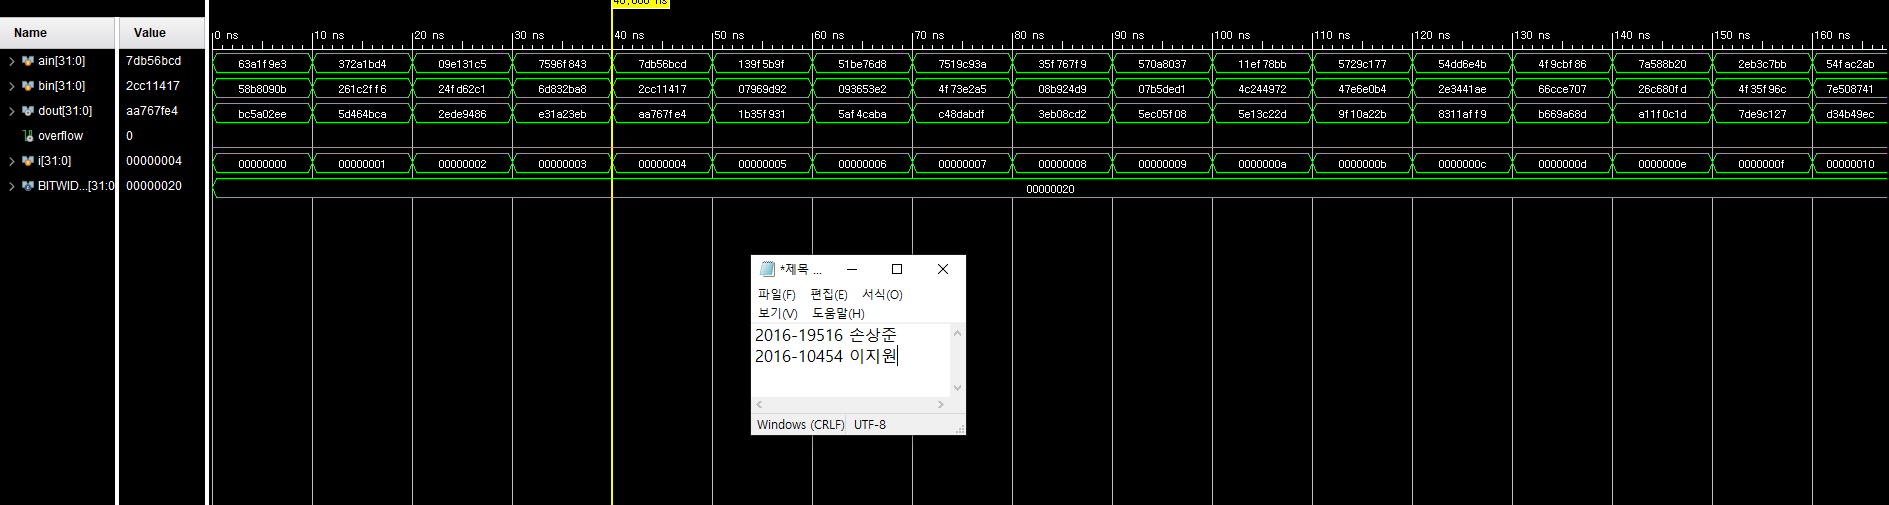
\includegraphics[width=1.0\textwidth]{fig/fig1.png}
	\caption{Testbench result of Adder}
\label{fig1}
\end{figure}

\subsection{Multiplier}
testbench에서 주어지는 ain, bin의 값은 0 ~ $2^{31}-1$ 까지의 임의의 값이다.
따라서, dout의 값은 최대 $2^{62}-2^{32}+1$ 이고, 이는 64bit로 만들 수 있는 최댓값인 $2^{64}-1$ 보다 작으므로 주어진 testbench에서는 overflow가 발생하지 않는다.
또한, ain, bin 이 가질 수 있는 최댓값인  $2^{32}-1$ 일때도 동일하게 overflow는 발생하지 않는다. 

\begin{figure}[ht]
	\centering
	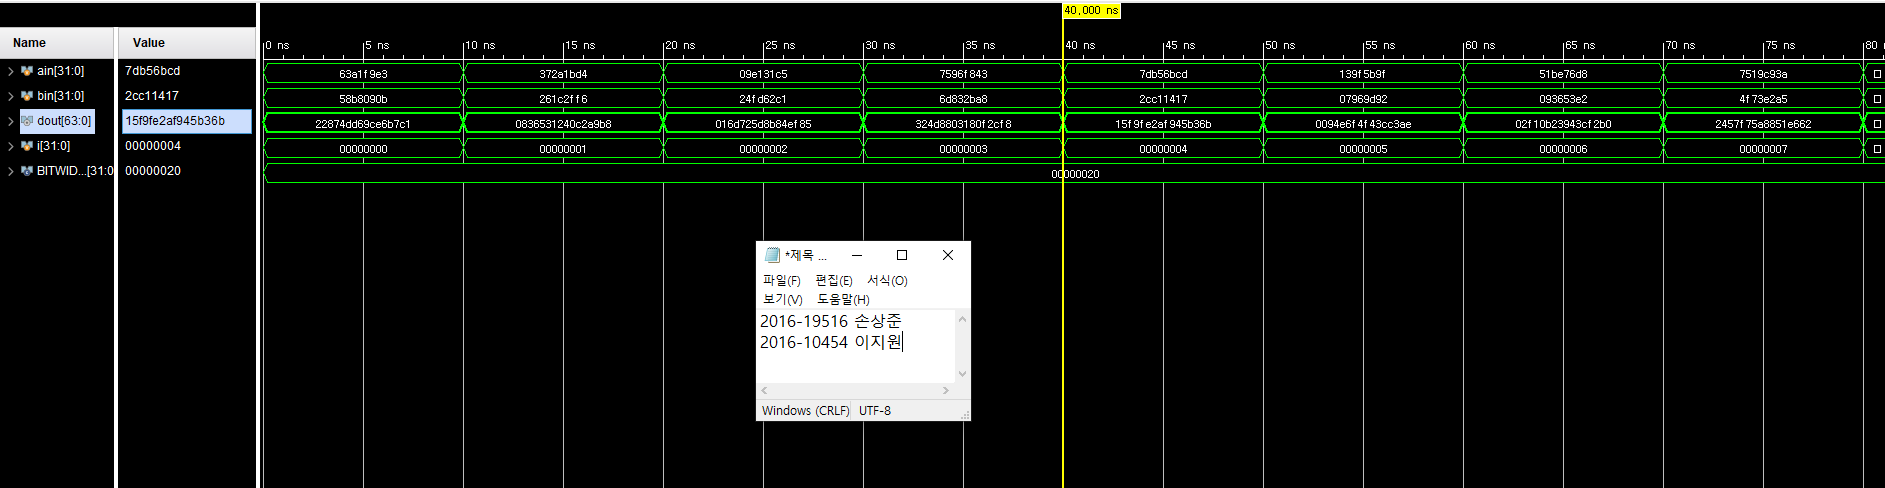
\includegraphics[width=1.0\textwidth]{fig/fig2.png}
	\caption{Testbench result of Multiplier}
\label{fig2}
\end{figure}

\subsection{Fused Multiplier}
testbench에서 clk, en값은 0으로 시뮬레이션 시작과 동시에 할당된다. 이후, 30ns에서 en값이 1로 변경된다. 또한, 주어지는 ain, bin의 값은 0 ~ $2^{31}-1$ 까지의 임의의 값이다. ain, bin의 값은 30ns에 할당되기 때문에, 30ns 이전에는 unknown으로 처리됨을 알 수 있었다
clk의 posedge는 5ns부터 10ns마다이기 때문에, dout의 값은 35ns이전에는 0(en이 0이기 때문에), 이후에는 단일 곱셈-누산기의 역할을 수행하였다.
특히, clk의 posedge에서만 en의 값이 읽히기 때문에, dout의 값이 0~5ns까지 unknown, 그 이후부터는 en의 값에 따른 정확한 결과값이 저장됨을 확인 할 수 있었다.

\begin{figure}[ht]
	\centering
	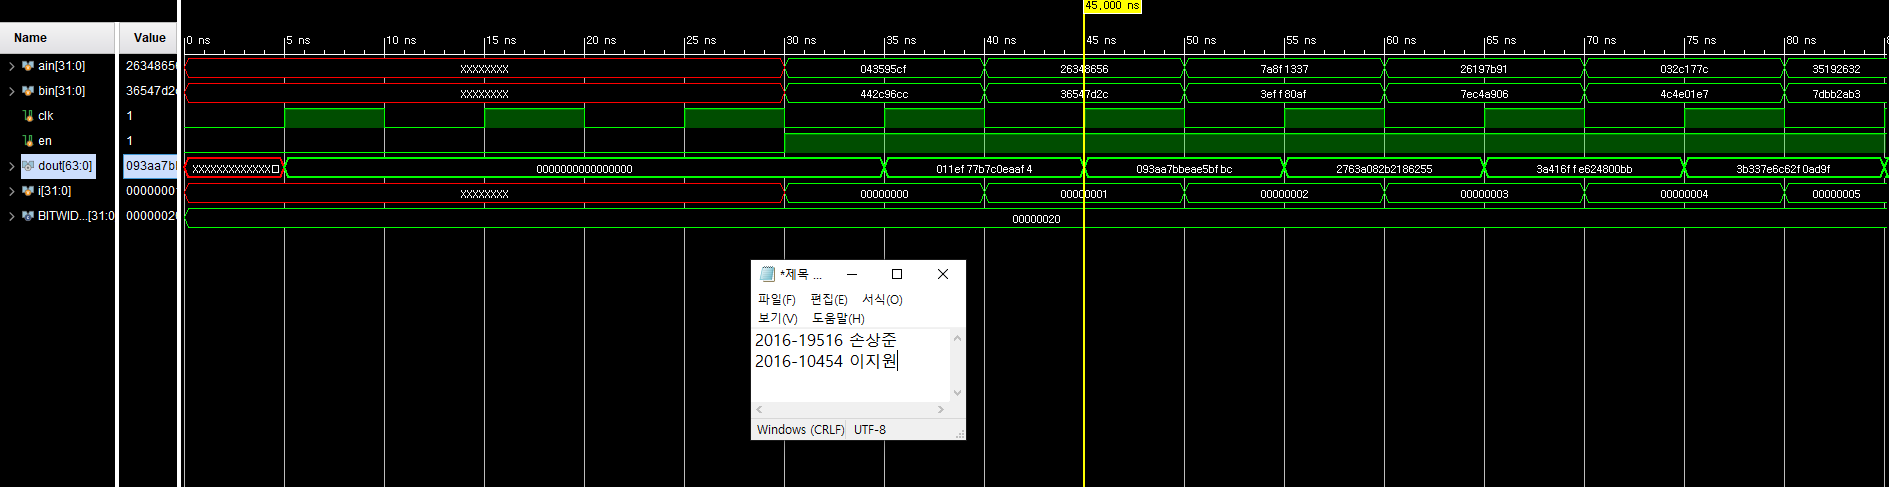
\includegraphics[width=1.0\textwidth]{fig/fig3.png}
	\caption{Testbench result of Fused Multiplier}
\label{fig3}
\end{figure}

\end{document}
